\documentclass{article}
\usepackage{graphicx}
\usepackage{wrapfig}
\usepackage{array}
\usepackage{url}
\usepackage{graphicx}
\usepackage{wrapfig}
\usepackage{float}
\title{Chapter four and seven case studies}

\author{Mohsen Tavakoli, Maan Joseph, Oluwaseyi Akinlade, Nima Moradianzadeh}

\begin{document}

\maketitle
\section{Case Study: Ann’s Rendezvous}
\subsection{Problem description}
In this assignment we aims to analyzing the packet capture and also collect the information from a suspected persons activities.
 
The following questions will help guide your investigation:
• Provide any online aliases or addresses and corresponding account credentials that
may be used by the suspect under investigation.
• Who did Ann communicate with? Provide a list of email addresses and any other
identifying information.
• Extract any transcripts of Ann’s conversations and present them to investigators.
• If Ann transferred or received any files of interest, recover them.
• Are there any indications of Ann’s physical whereabouts? If so, provide supporting
evidence.
Network:
• Internal network: 192.168.30.0/24
• DMZ: 10.30.30.0/24
• The “Internet”: 172.30.1.0/24 [Note that for the purposes of this case study, we are
treating the 172.30.1.0/24 subnet as “the Internet.” In real life, this is a reserved nonreturnable
IP address space.]
Evidence: Investigators provide you with a packet capture from Ann’s home network,
“evidence-packet-analysis.pcap.” They also inform you that in the course of their monitoring,
they have found that Ann’s laptop has the MAC address 00:21:70:4D:4F:AE
\subsection{Experiment}
\subsubsection{simulation}
In order to emulate the network of the problem we used GNS3. GNS3 can be used in order to emulating the complex network. Virtual devices and actual devices can be set by this software\cite{amyot2014system}.


\subsubsection{Tools Used}
To conduct the experiment we mainly used two tools interacting together. The first tool we used to setup the network is GNS3 and the second tool we used is Wireshark to analyze the packets captured during normal network communication.


\subsubsection{GNS3 (Graphical Network Simulator-3)}
GNS3 is a network software emulator. It facilitates the simulation of network traffic using real and virtual devices. GNS3 was initially intended to simulate Cisco routers and switches but then it was expanded to support other platforms as well and today it is used emulate various complex networks.  GNS3 Was used in our experiment to setup and emulate network traffic. 


We are able to create routers and switches and add different computers on the network. Doing so, we were able to communicate with different computers across different switches \cite{hassine2014toward}.


\subsubsection{Wireshark}
Is a network tool that is used to analyze packets transmitted over a computer network. It is open source and supported across many platforms. The way it operates is very similar to TCPDUMP however it has a graphical user interface to make it easier for the network engineer to troubleshoot the network \cite{orebaugh2006wireshark}.


For the sake of our experiment, a capture tool is added between the two routers shown in network topology that captures traffic between two routers. The capture tool capture the network packets being transmitted over the network for wireshark in order for them to be analyzed.

\subsection{Network Topology}

The emulated topology(Figure.\ref{fig:TPLGY}) consists:

\begin{itemize}
	
	\item Two Cisco c7200 Routers (R1 and R2)
	\item Five Cisco Ethernet Switches (SW1 to SW5)
	\item Seven Virtual Machines (PC1 to PC7)
	\item Two Microsoft Loopback Adaptor 
\end{itemize}

The PCs are connected to the switches which are connected to one of the Reouters fast ethernet Ports:


\begin{itemize}
	
	\item Sw1 is configured on R1 interface f1/0 and 192.168.30.0/24
	\item Sw2 is configured on R1 interface f2/0 and 172.30.1.0/24
	\item Sw4 is configured on R1 interface f3/0 and 1923.164.137.0/24
	\item Sw3 is configured on R2 interface f1/0 and 192.122.52.0/24
	\item Sw5 is configured on R2 interface f2/0 and 190.168.136.0.24/24
\end{itemize}

R1 and R2(Cisco c720 Routers) are connected together on the fast Ethernet port 0:10.30.30.254 and 10.30.30.253 respectively.The R1 is active router for Sw1 ,Sw2 and SW4 and R2 is active Router for S5 and Sw3. Additionally, the virtual machines use Dynamic Host Configuration Protocol(DHCP) in order get IP address. This Protocol can be used in order to set the IP host and its related configuration information.


\begin{figure}[H]
	\begin{center}
		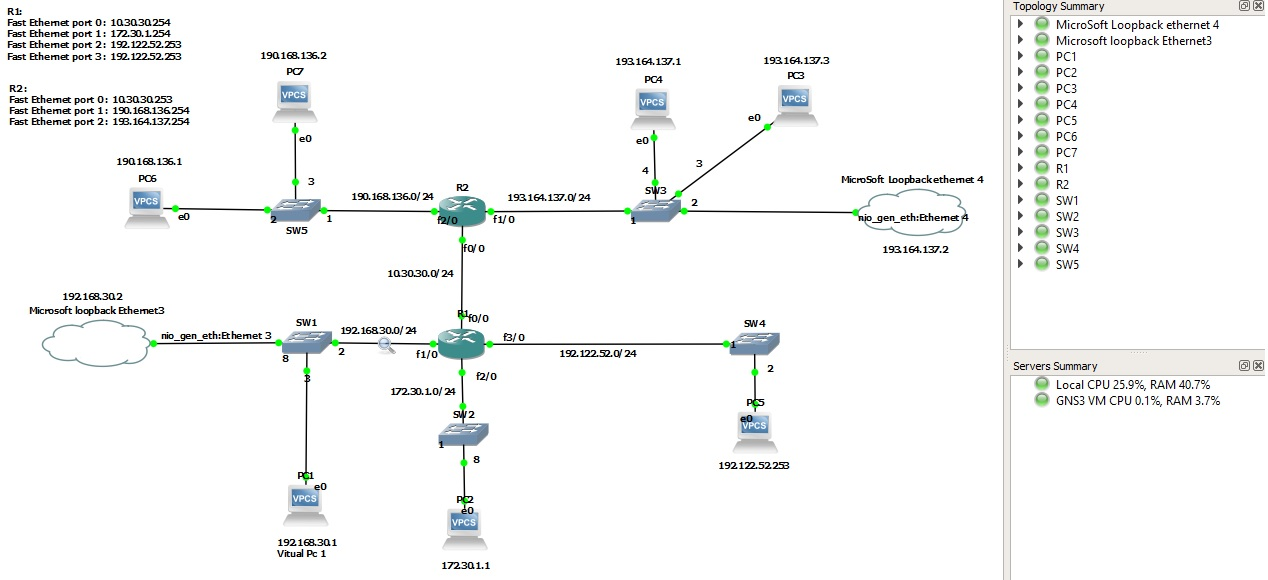
\includegraphics[width=0.6\textwidth]{Topology.jpg}
	\end{center}
	\caption{\small  Our Simulated Network Topology\newline}
	\label{fig:TPLGY}
\end{figure}
\subsection{Km-test Loopback}

Microsoft Loopback Adapter has some capabilities that can be used in our model. Firstly, it can be used for virtual network protecting by using Internet Connection Firewall. Secondly, Designer also can use it to share the files independently and design host-to-guest networking. Lastly, providing the Network Address Translation (NAT) and sharing connection to Internet are other capabilities of this software.\\
We installed MS Loopback as an additional Network adapter on the computer. In following, we described how we installed Microsoft Loopbaack Adapter:
In the Device Manager panel click on Action and choose the Add legacy Hardware. Now the installation page is opened (Figure.\ref{fig:KMINS}) . For more information about installation you can check this website:\\
	\url{https://technet.microsoft.com/en-us/library/cc708322(v=ws.10).aspx}


\begin{figure}[H]
	\centering
		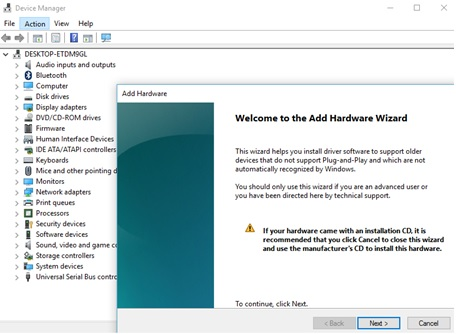
\includegraphics[width=0.6\textwidth]{LoopBackIns1.jpg}
	
	\caption{\small Microsoft KM-test Loopback Adapter Installation\newline}
	\label{fig:KMINS}
\end{figure}


NOTE: just note that you choose the Microsoft KM-TEST Loopback Adapter on the Network Adapters section (Figure.\ref{fig:KMINS2}) .


\begin{figure}[H]
	\begin{center}
		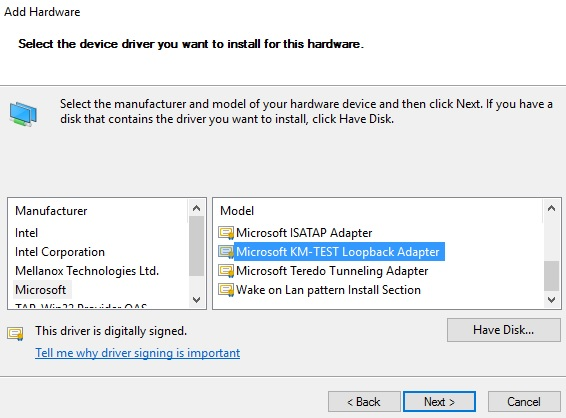
\includegraphics[width=0.6\textwidth]{LoopBackIns2.jpg}
	\end{center}
	\caption{\small Network Adapters section \newline}
	\label{fig:KMINS2}
\end{figure}


In Figure.\ref{fig:StatusEth}, you can see that there are two Real nodes configurations which are connected to the networks 193.164.137.0 and 192.168.30.0 in cloud figure.\\


These two LAN module in GNS3s simulated network are connected to a real PC and have different topologies for their connection. Figure.\ref{fig:StatusEth} shows that Ethernet 3 used the IP address 192.168.30.2 and Ethernet 4 using 172.30.1.2. Furthermore, both have same Gateway (255.255.255.0)


\begin{figure}[H]
	\begin{center}
		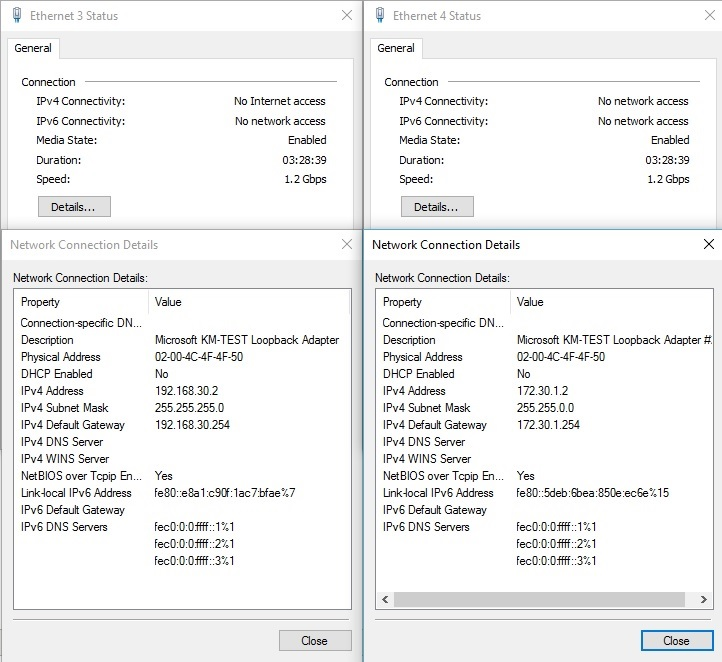
\includegraphics[width=0.6
\textwidth]{Ethernet.jpg}
	\end{center}
	\caption{\small Ethernets Status \newline}
	\label{fig:StatusEth}
\end{figure}


Linux PCs: When we created the network, we emulated computers running on Linux platforms. The PC's were used to communicate with each other by sending and receiving packets from each other in order for Wireshark to capture and analyze them. The PC's were configured with these below network configuration:\newline
***.***.***.***/subnet\newline
***.***.***.***(gateway)

\begin{figure}[H]
	\begin{center}
		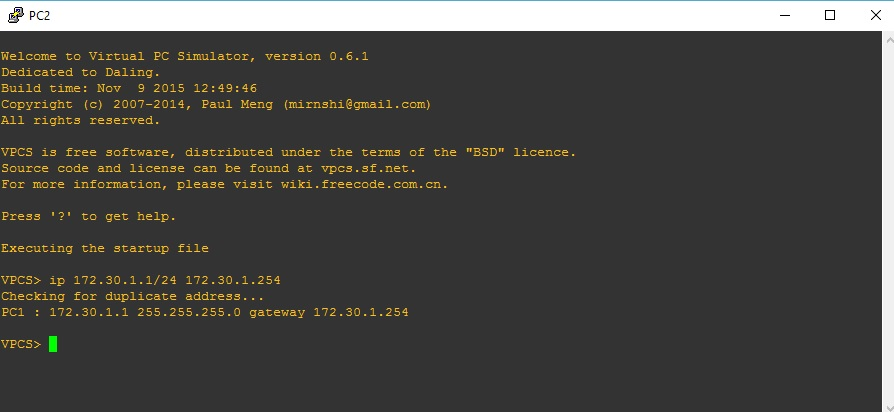
\includegraphics[width=0.6
\textwidth]{VPC.jpg}
	\end{center}
	\caption{\small  \newline}
	\label{fig:VPC}
\end{figure}
Vpcs in Fig 5 is a virtual pc simulator found in GNS3, used for testing in GNS3 with ping and traceroute capabilities. Virtual pcs command : IP [address] [/mask] [gateway].The ip address of the virtual pc 2 is configured by entering the ip command then assigning 172.30.1.1/24 as the ip address and subnet then 172.30.1.254 as the gateway. The console then checks if it is a duplicate address and ping command is then used to test connectivity.

\subsection{Ethernet Switches}
We configure the switches and grant access to all the ports for future computers.
In this page, we can set the switch for different cases in the lab. We used the
default mode which consists of 8 ports (Figure 6).

\begin{figure}[H]
	\begin{center}
		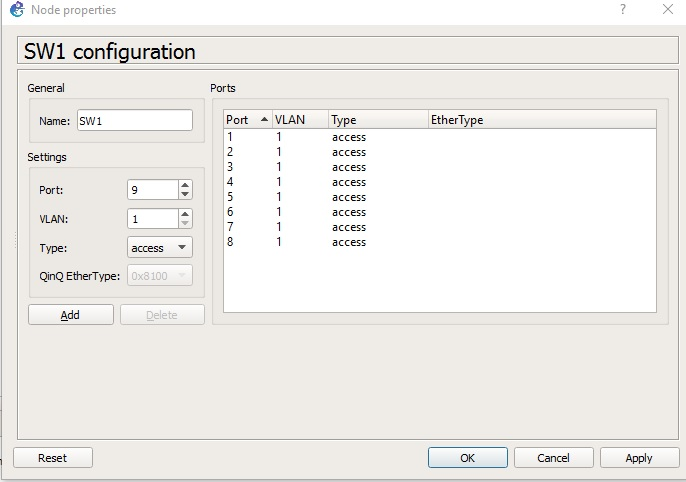
\includegraphics[width=0.6
\textwidth]{Switchconf.jpg}
	\end{center}
	\caption{\small  \newline}
	\label{fig:Prd}
\end{figure}

\subsection{Routers configurations}

Figure.\ref{fig:Termconf} shows how an IP can be configured on a Cisco router interface. The first step, the router enabled to turn on privileged commands (If the password has been set for the router after entering enable the command line asked you to enter the password). Secondly, The second command (configure terminal) is used to enter to global configuration mode. Then you need to enter to the fast Ethernet Interface configuration mode, and the IP address and Gateway will be written in the next step. By default, the interface is "Administratively Down" means that the port is closed. So lastly, we used "no shutdown" command to enable it.

\begin{figure}[H]
	\begin{center}
		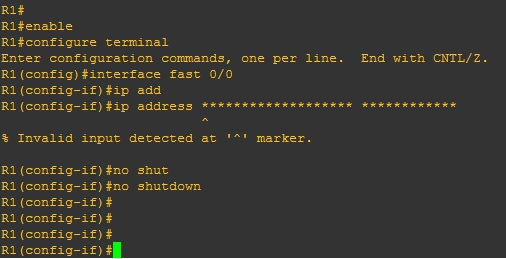
\includegraphics[width=0.6
\textwidth]{Terminalconf.jpg}
	\end{center}
	\caption{\small Enter An IP to the Cisco Router \newline}
	\label{fig:Termconf}
\end{figure}

We configure each Router Interface.\\


\begin{figure}[H]
	\begin{center}
		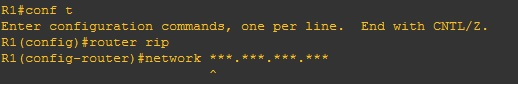
\includegraphics[width=0.6
\textwidth]{RouterRip.jpg}
	\end{center}
	\caption{\small  \newline}
	\label{fig:Prd}
\end{figure}
\subsection{Routing information Protocol (Rip)} Fig 8 displays the routing Information Protocol. The Rip uses hop counts as a metric to determine the best path to a network and also prevents routing loops. The "router configuration terminal" command is first entered to start the rip process, then the "router rip" command is entered in the console, The "network *.*.*.*.*.*.*.*.*.*" command is used to assign networks that would participate in the rip process. The "show ip rip database" command displays all the networks in the RIP database. The "show ip protocols" displays the global configurations of the Rip process which include timers, network etc.

Router 1 Configuration: (do the exact thing for the other router

\begin{figure}[H]
	\begin{center}
		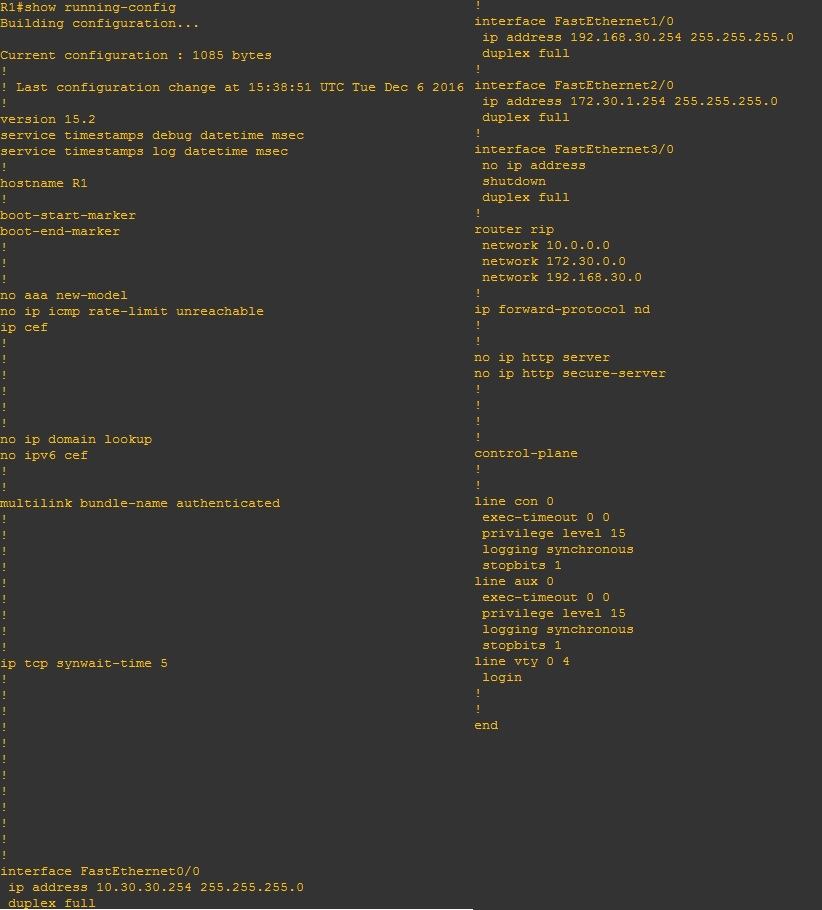
\includegraphics[width=0.6
\textwidth]{Routerconfig.jpg}
	\end{center}
	\caption{\small  \newline}
	\label{fig:Prd}
\end{figure}


\subsection{Wireshark Packets Capturing}
When computers are communicating over the network, we used Wireshark to capcture the packets being sent back and forth. As shown in Figure 10 below list of packets captured, each packet holds significant of information, for example the sender and receiver. Each packet is stamped with time captured, source of the sender in ipv4 address format and destination address also in ipv4 along with the sending protocol. From the list pange, we are able to click on any packet and find more details about it in the tree view or byte view panes. 

\begin{figure}[H]
	\begin{center}
		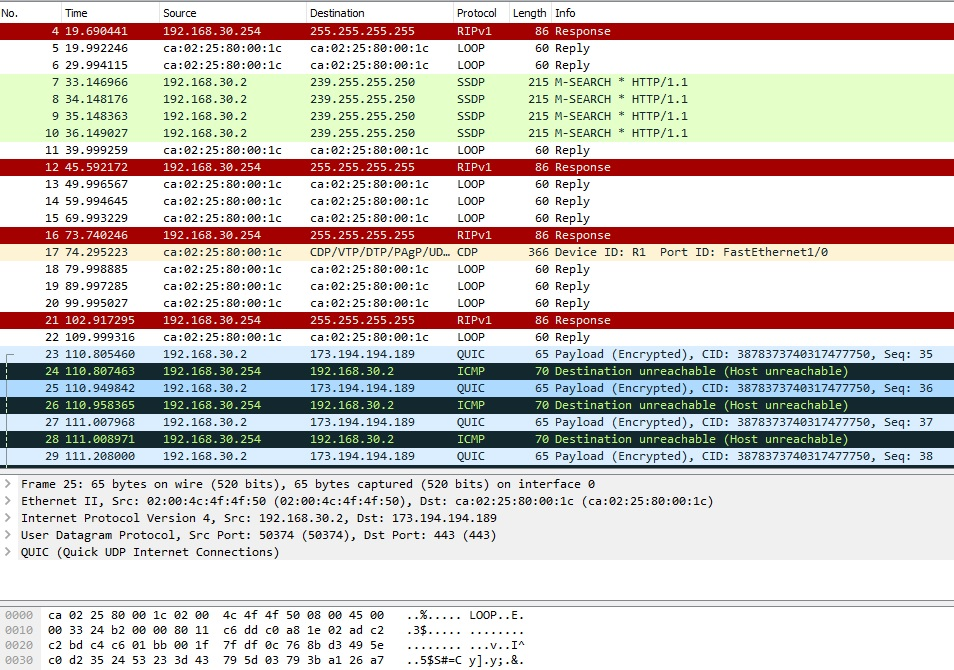
\includegraphics[width=0.6
\textwidth]{wireshark.jpg}
	\end{center}
	\caption{Packets captured by Wireshark}
	\label{fig:Prd}
\end{figure}

\subsection{Protocol Hierarchy}
Fig 11. displays the protocol heirachy of the captured packets. It is a tree of all protocols in the capture, with each row containing the statistical values of one protocol.The percant packets and bytes columns also contain bar graphs. Multiple protocols can be found in a single packet and it can also contain the same protocol more than once. This data can be copied using the copy button as CSV or YAML.
\begin{figure}[H]
	\begin{center}
		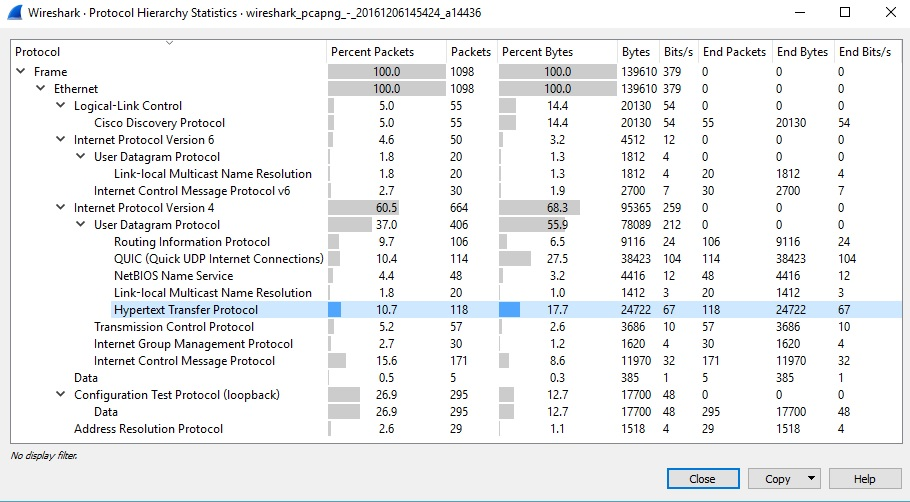
\includegraphics[width=0.6
\textwidth]{Hierarchyst.jpg}
	\end{center}
	\caption{\small  Protocol Heirachy statistics window\newline}
	\label{fig:Prd}
\end{figure}


\subsection{TCPFlow - Data stream analysis}
Here we examine Wireshark capturing result and analyze the TCP flow. As you can see from figure 12, the conversation between the computers on the network is about Grammarly that is originated from 54.221.52.117 to destination 137.207.64.60. For the output we used TCP flow with the appropriate port setting and reconstructed the data streams as shown in figure 13 with plain paragraphs that are readable. 
\begin{figure}[H]
	\begin{center}
		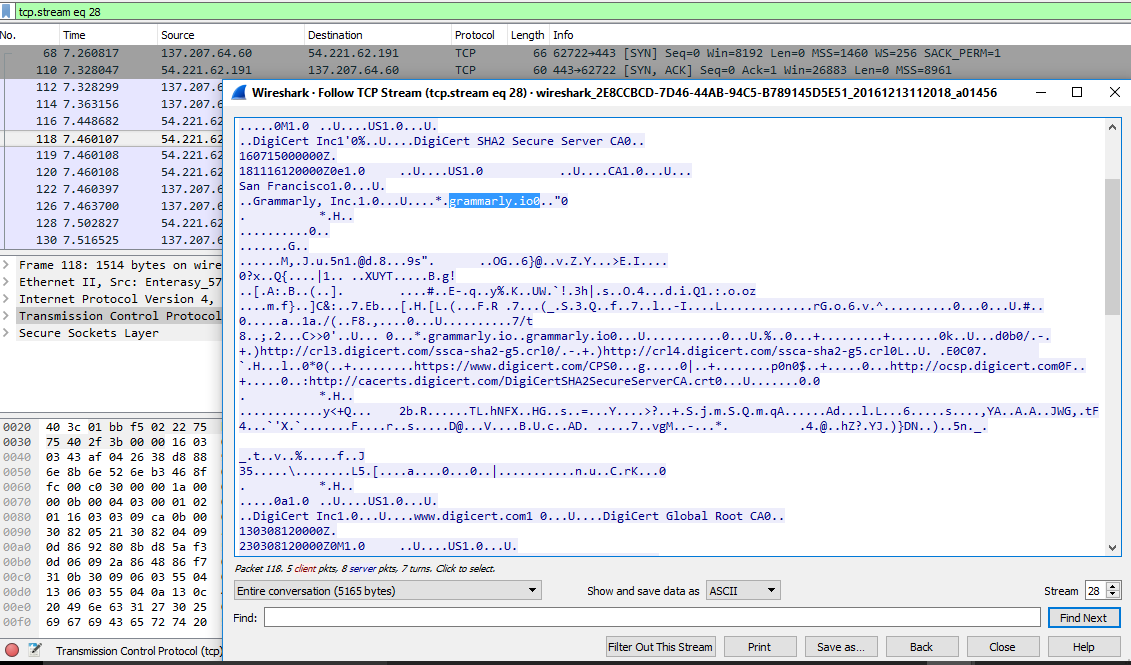
\includegraphics[width=0.6
\textwidth]{TCPFLOW1.png}
	\end{center}
	\caption{TCPFlow}
	\label{fig:Prd}
\end{figure}

\begin{figure}[H]
	\begin{center}
		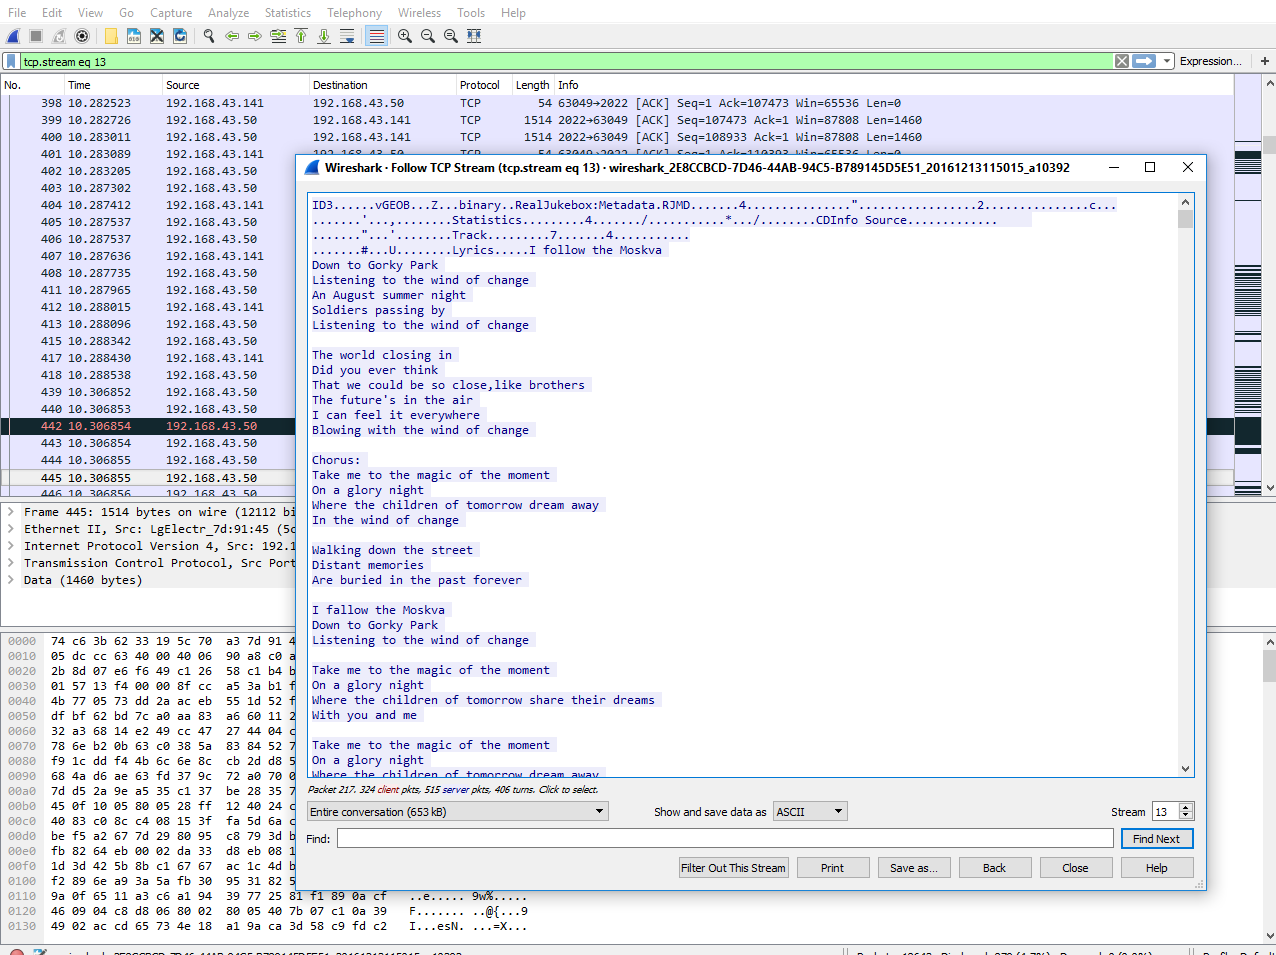
\includegraphics[width=0.6
\textwidth]{TCPFLOW2.png}
	\end{center}
	\caption{TCPFlow Data reconstructed}
	\label{fig:Prd}
\end{figure}

\subsection{Finding \textit{{Ann}}}
We used NetworkMiner in order to conduct this step. Networkminer is a network forensic tool that can be used as a network sniffer with a purpose to detect operating systems, open ports and hostnames without putting any traffic on the network. The main purpose of NetworkMiner is to collect data about the hosts on the network. NetworkMiner is capable of parsing files and certificates from the PCAP file \cite{crenshaw2008osfuscate}.

The PCAP file we obtained was opened in NetworkMiner, then the information was automatically filled in NetworkMiner that were extracted from the PCAP file. As you can see from Figure 15, "Hosts" tab lists all the IP address of the host transmitted IP traffic in the packet capture. 
\begin{figure}[H]
	\begin{center}
		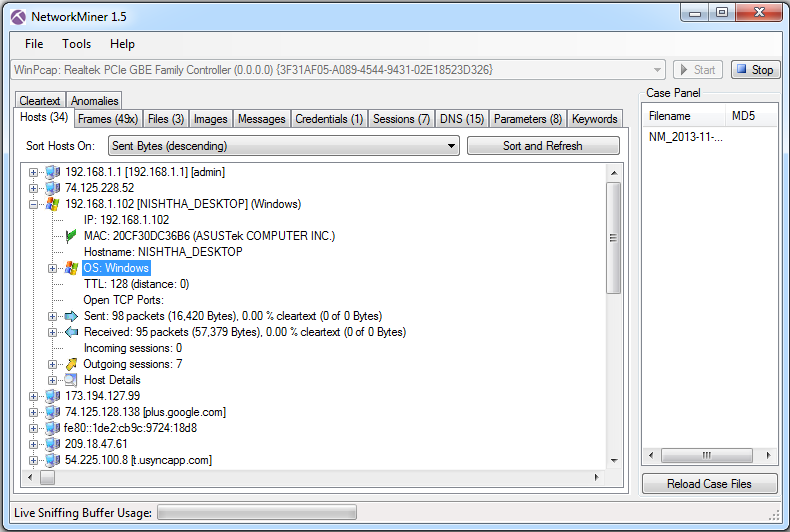
\includegraphics[width=0.6
\textwidth]{FINDINGANN1.png}
	\end{center}
	\caption{List of devices discovered on the network by NetworkMiner. We opened the PCAP file in network to interpret the results. }
	\label{fig:Prd}
\end{figure}

\begin{figure}[H]
	\begin{center}
		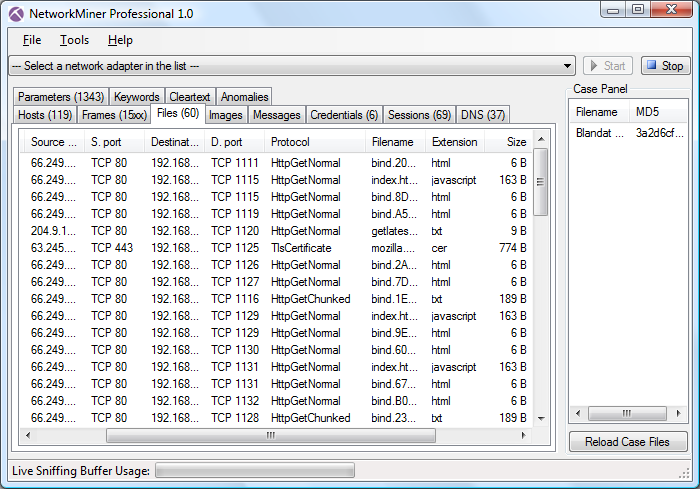
\includegraphics[width=0.6
\textwidth]{FINDINGANN2.png}
	\end{center}
	\caption{"Files" tab of the requests being made from the source computer to the network along with the port being used and the network protocol that are embedded inside the captured packet.}
	\label{fig:Prd}
\end{figure}

\subsection{File Carving}
This section begins here
\begin{figure}[H]
	\begin{center}
		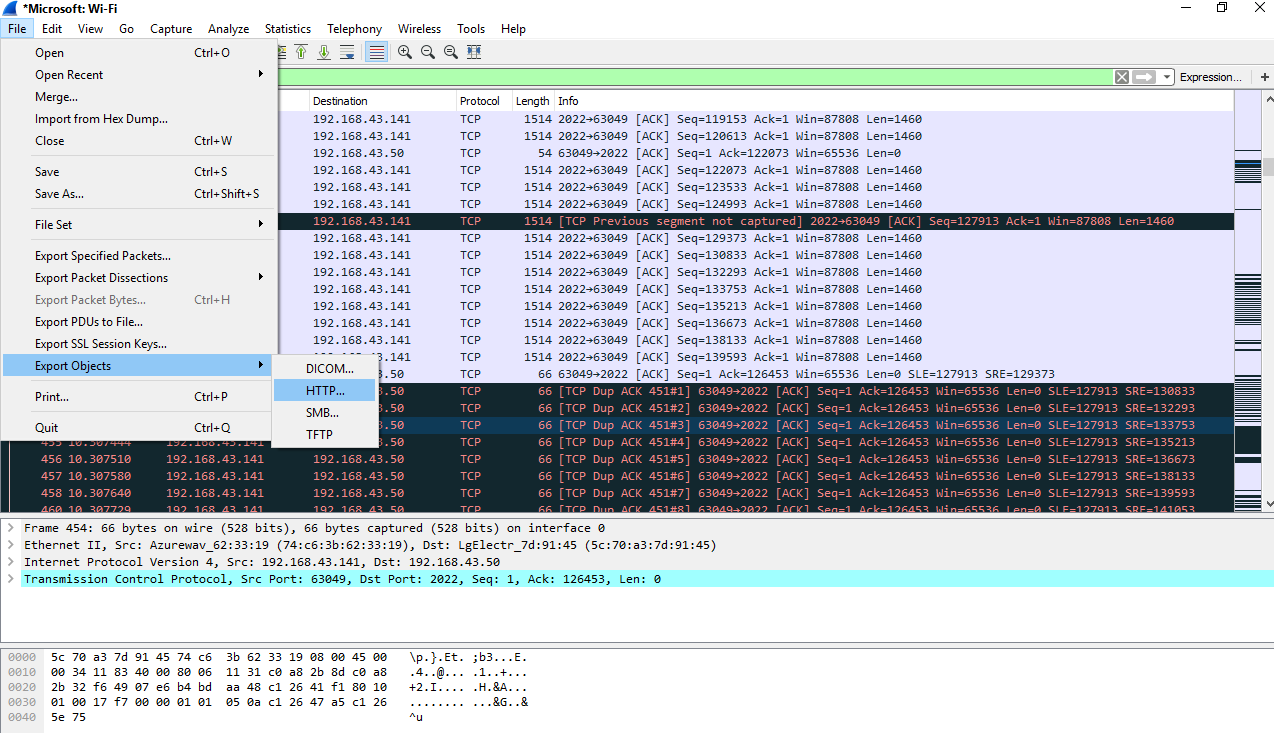
\includegraphics[width=0.6
\textwidth]{FILECARVING1.png}
	\end{center}
	\caption{test1.}
	\label{fig:Prd}
\end{figure}

\begin{figure}[H]
	\begin{center}
		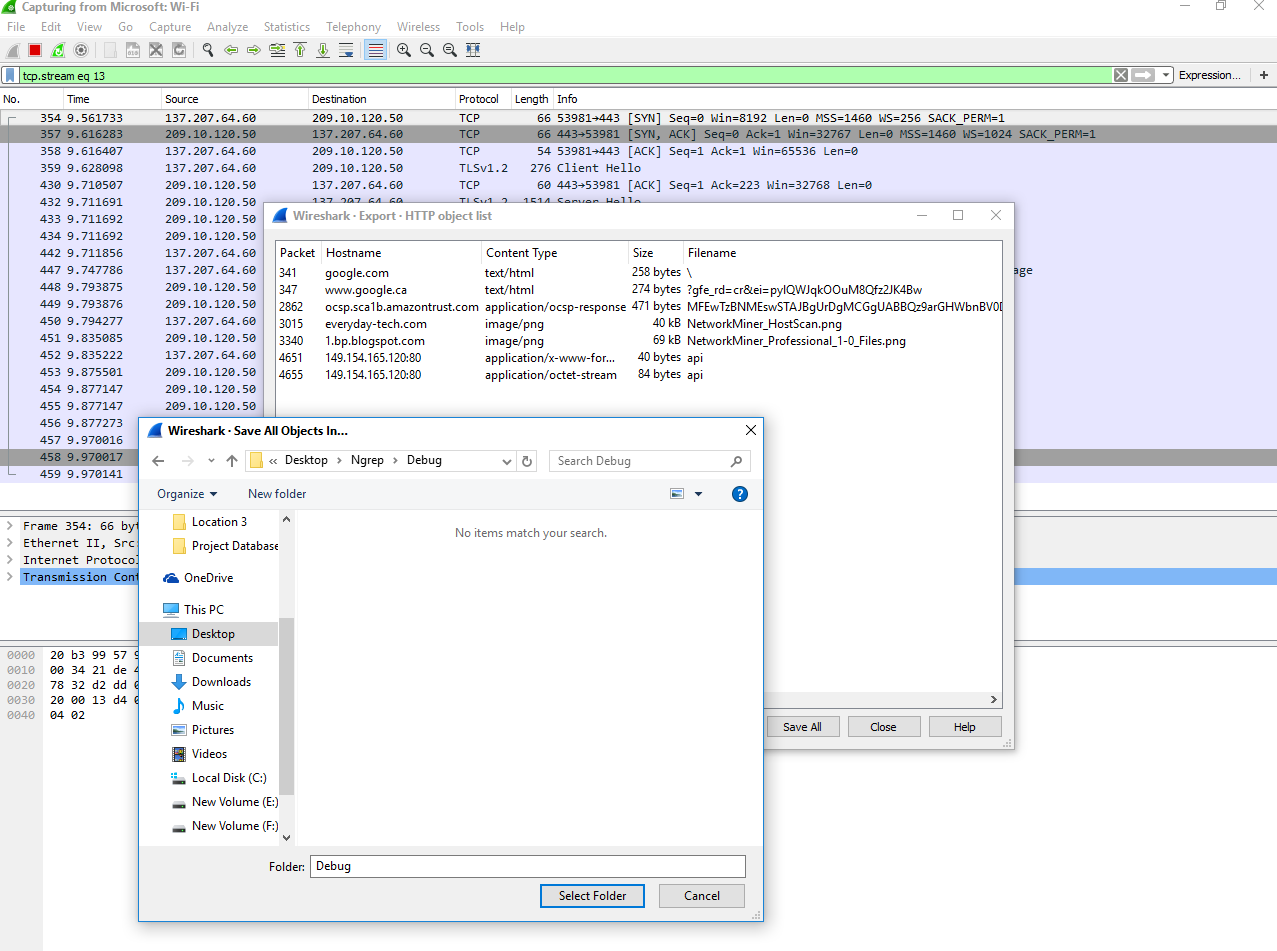
\includegraphics[width=0.6
\textwidth]{FILECARVING2.png}
	\end{center}
	\caption{test1.}
	\label{fig:Prd}
\end{figure}


\section{Case Study: Interoptic Saves the Planet}


\subsection{Problem statement}




\subsection{What is the Snort?}
Snort is an open-source Intrusion Prevention Systems (IPS) , however first it designed to be Intrusion Detection System). It is able to analyze the protocol,search and match the content\cite{carr_2007}. \\

\subsection{Snort Installation}
We installed snort tool and configured it on our wireless module in order to connect to the network.
To use this software you need to install both installation software and the rules from the \url{https://www.snort.org/downloads}. There are three types of rules for downloading.\\

you need to install the snort by snort installer and then the Rules file needs to be extracted to the rules folder in directory of the installed snort.then you need to For more information about installation of snort on windows you can visit this website \url{https://www.sans.org/security-resources/idfaq/running-snort-under-windows/6/4}.\\

\subsubsection{Configuration of rules:}
We also specified each port in this section for the snort to listen through the network, in this case we set snort to listen to any port through the network. The Figure.\ref{fig:Ipconf} shows the changes in "snort.conf" file in order to listen to any port.

\begin{figure}[H]
	\begin{center}
		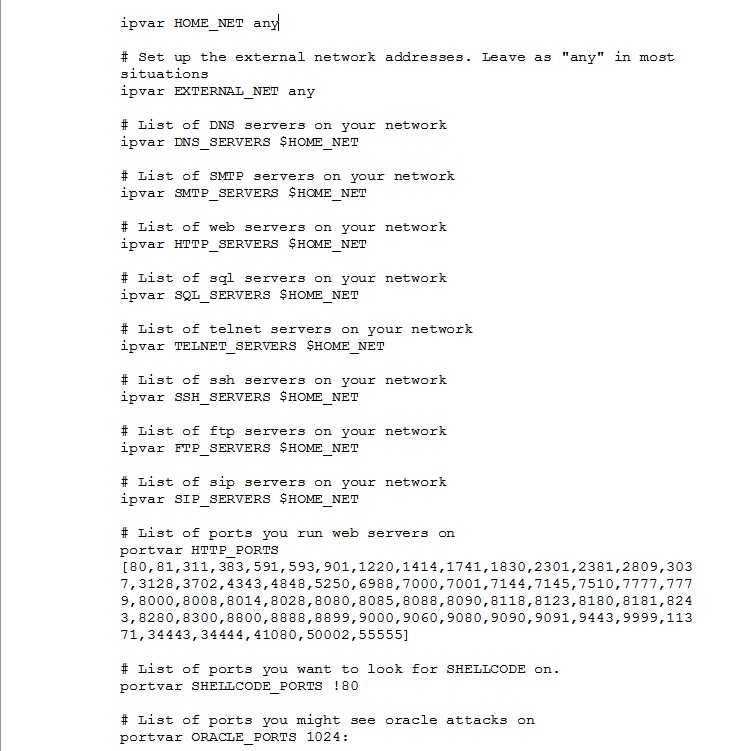
\includegraphics[width=0.6
		\textwidth]{Ipconf.jpg}
	\end{center}
	\caption{Configured Ip addresses}
	\label{fig:Ipconf}
\end{figure}

When the installation finished, to make sure that installation is completed we used the "Snort.Exe -W" (Figure.\ref{fig:SnortIns}). This figure shows that we have three available interface. Their physical addresses and Ip addresses  will be shown by this command. In our cases number 2 is  wireless.


\begin{figure}[H]
	\begin{center}
		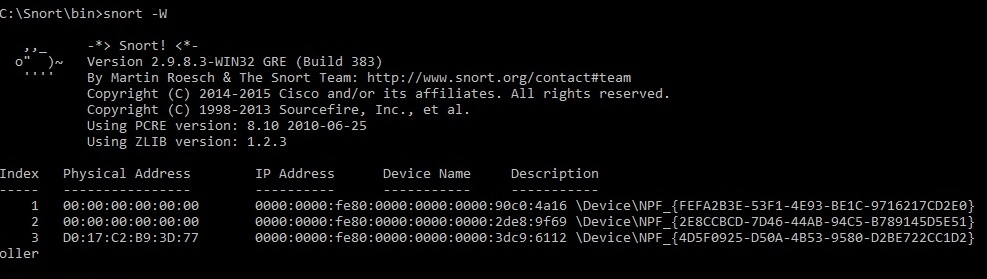
\includegraphics[width=0.6
\textwidth]{SnortIns.jpg}
	\end{center}
	\caption{Snort Installation}
	\label{fig:SnortIns}
\end{figure}





\subsection{Rules and alert:}

We program alert for the snort to do alert number 1**1-3 through the connections generated through the each specific protocols. Bare that in mind for the training purpose of this case study we listen to each protocol. The configuration happened in local.rules in /etc folder (Figure.\ref{fig:Localnet}) .

\begin{figure}[H]
	\begin{center}
		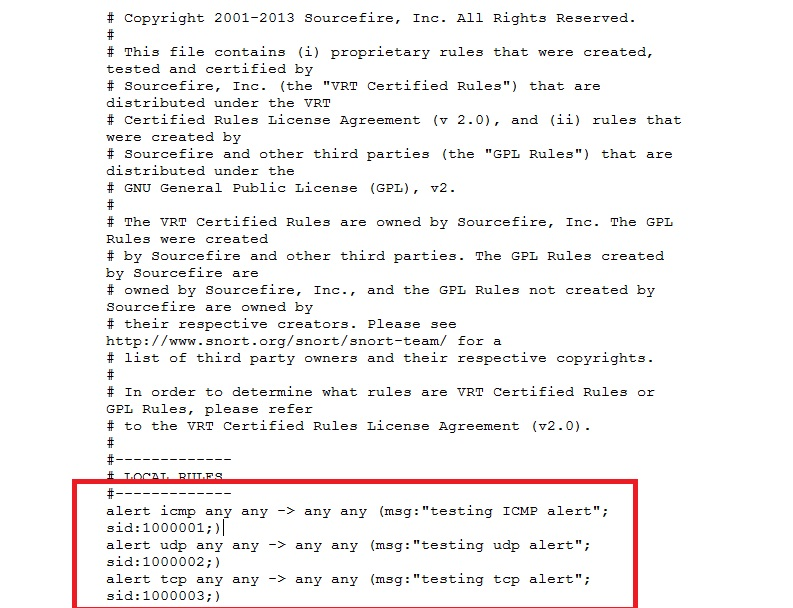
\includegraphics[width=0.6
\textwidth]{Localnet.jpg}
	\end{center}
	\caption{Configured local rules over the network}
	\label{fig:Localnet}
\end{figure}






\subsection{Setting interface 2}
This is wireless module of the pc connected to the network. As it mentioned the interface number 2 is our wireless module. We initialize the snort to listen to all the specific ports that you can see in the Figure.\ref{fig:Ipport} and ip addresses in order to see if someone is trying to connect to our network and see if there are any attacks are happening on our network and ports.

\begin{figure}[H]
	\begin{center}
		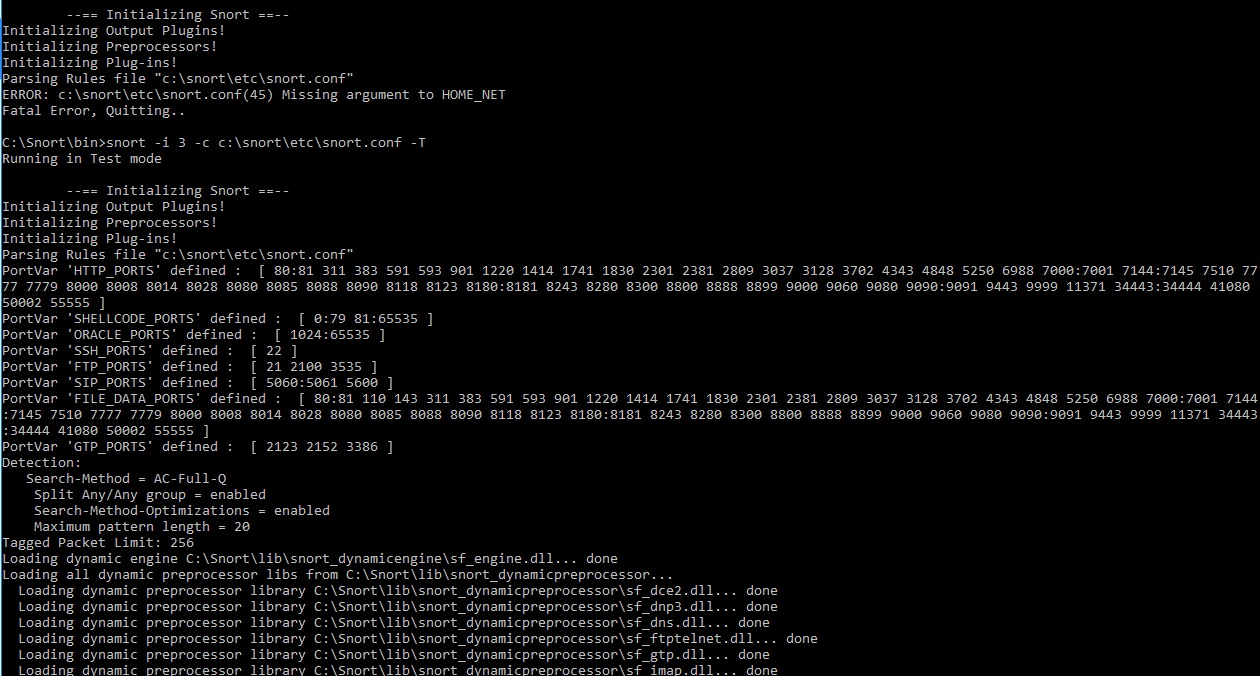
\includegraphics[width=0.6
			\textwidth]{portip.jpg}
	\end{center}
	\caption{Configured 1 - on ports and ip addresses}
	\label{fig:Ipport}
\end{figure}


Start Capturing:
By running the command:
Snort -i 2 -c \url{c:\snort\lib\snort.conf -A console}

\begin{itemize}
	
	\item -i select the interface * is the number (in this case is  2)
	\item -c which allow us to choose which configuration file we want to use in this case is given the address in the next section
	\item C:\ (we gave the address of our configuration in this part which is located in ‘lib’ folder
	\item -A console we command the snort to run the command and show us the results of our command in the same CMD.exe as given below. 
\end{itemize}



 


\begin{figure}[H]
	\begin{center}
		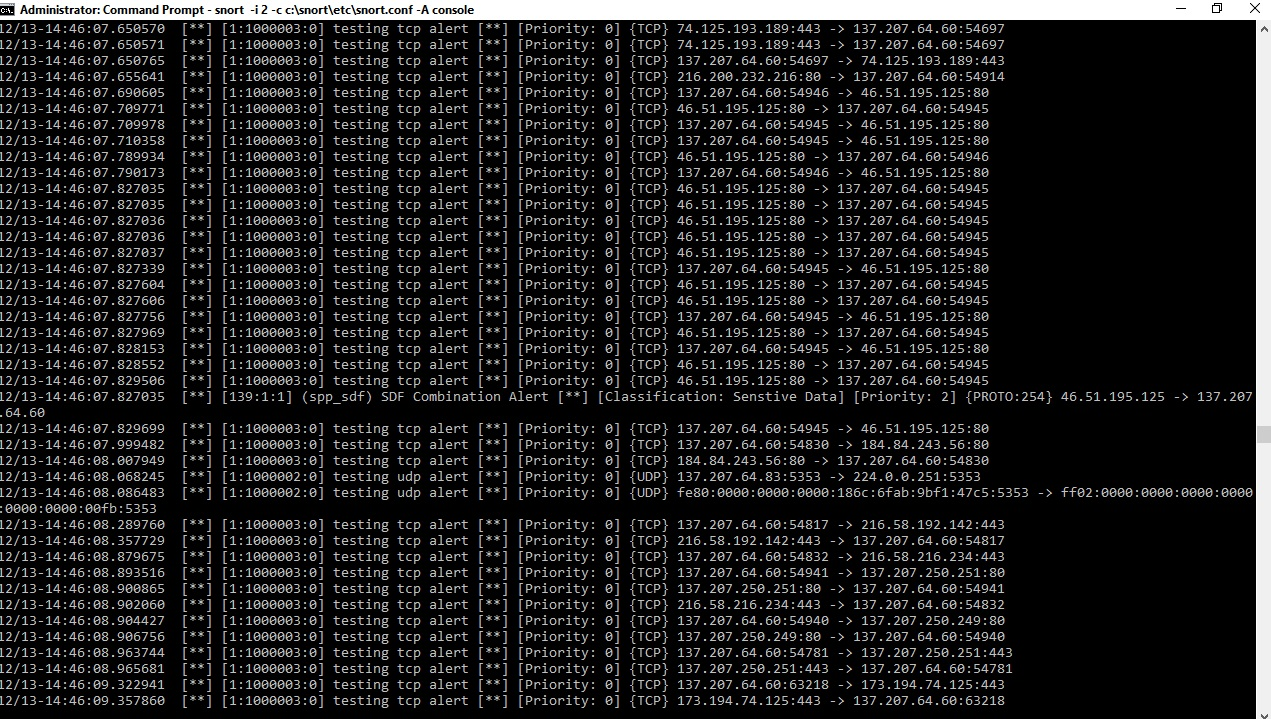
\includegraphics[width=0.6
\textwidth]{Conf4.jpg}
	\end{center}
	\caption{configured 4 - Captured packets over the network}
	\label{fig:Conf4}
\end{figure}


This figure show the alerts that we configured which were given in last section with *1-3 numbers for each network protocols.
Results:
After we finished our packet capturing snort via command CRTL+C, snort will give you a very specific result of what had happened in the CMD which is shown below.

\begin{figure}[H]
	\begin{center}
		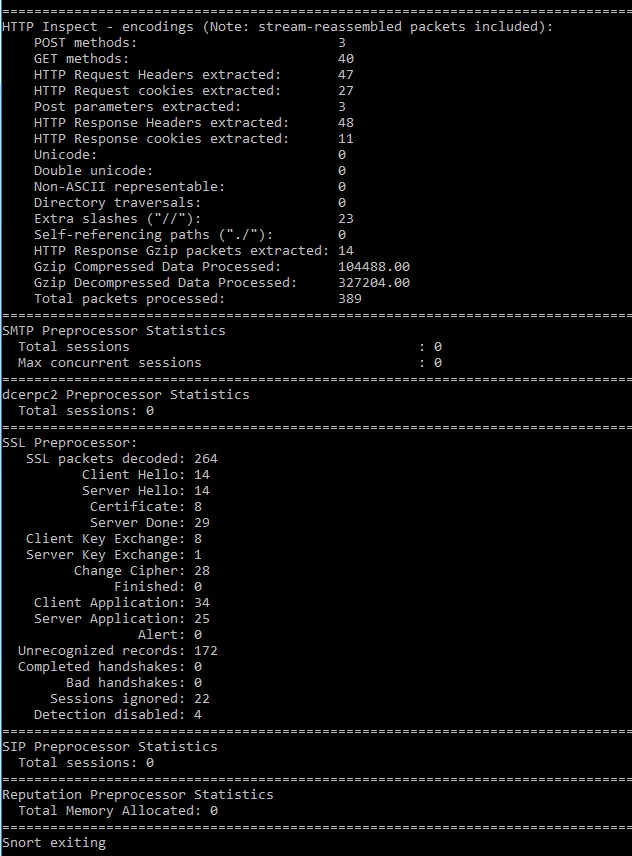
\includegraphics[width=0.6
\textwidth]{Res1.jpg}
	\end{center}
	\caption{HTTP inspect results over the given rules}
	\label{fig:Res1}
\end{figure}

Other results:

\begin{figure}[H]
	\begin{center}
		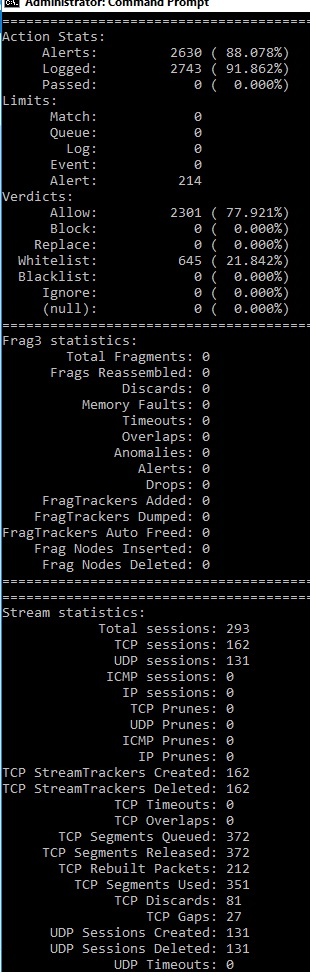
\includegraphics[width=0.3
\textwidth]{Res2.jpg}
	\end{center}
	\caption{Results over capturing 1.2}
	\label{fig:Res2}
\end{figure}


Other results:

\begin{figure}[H]
	\begin{center}
		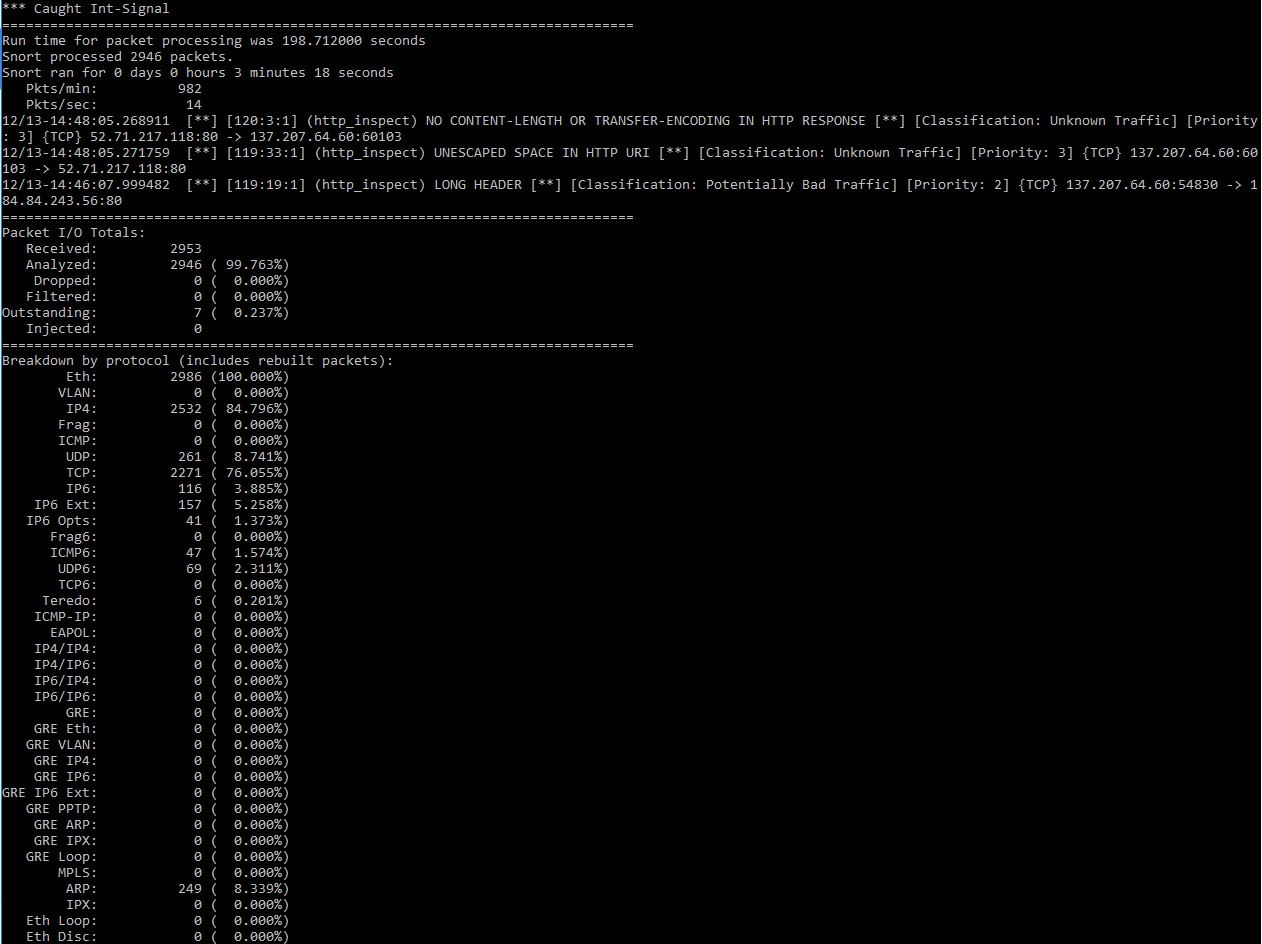
\includegraphics[width=0.6
\textwidth]{Res3.jpg}
	\end{center}
	\caption{Saved Results of over the time of capturing the packets}
	\label{fig:Res3}
\end{figure}

At the end snort will give us how many packets were captured, how many of them were the get methods over the network (use the picture in order to expand the report my friends)
\newpage
\tableofcontents
\bibliographystyle{ieeetr}

\bibliography{Kent-Case-Study1}
\end{document}
